\documentclass[12pt]{article}
\usepackage{amsmath} % flere matematikkommandoer
\usepackage{amssymb}
\usepackage[utf8]{inputenc} % æøå
\usepackage[T1]{fontenc} % mere æøå
\usepackage[danish]{babel} % orddeling
\usepackage{verbatim} % så man kan skrive ren tekst
\usepackage[all]{xy} % den sidste (avancerede) formel i dokumentet
\usepackage{graphicx}
\usepackage{listings}
\usepackage{appendix}


\title{Mobil-applikation til administration af webhosting-platform\\Projektkursus Systemudvikling 2014\\Delrapport 4}
\date{04-06-2014}
\author{Nicklas Warming Jacobsen 230891\\Christian Enevoldsen 020691\\Simon Warg 180489\\Robert Rasmussen 050394}

\lstset{
  breaklines=true,                 % sets automatic line breaking
}

\begin{document}
\maketitle
\begin{center}
  Instruktor: Kasper Passov
\end{center}
\newpage
\tableofcontents
\newpage
\section{Abstract}
The following report explains how the development of an application for both Android and iOS is created for and with the company Surftown. Surftown is a danish web-hosting company, with mainly scandinavian (Danish, Swedish and Norwigian) customers, which offers three services: Web-hosting, E-mail hosting and domain-name registration, plus a web-based controlpanel to allow Surftown's customers to configurate their acquired services. However Surftown wishes a smartphone application, to enable their customers to access parts of the functionality in their controlpanel, mainly informational functions.
One of Surftowns requirements for this project are that the application is programmed native to Android and iOS. We have therfore split the projekt group in two sub-groups containen two persons in each to focus respectively on the iOS application development and the Android application development. We use the same Surftown API and share some ressources between the Android application and the iOS application, and with this in mind we have created three git repositories; one for the iOS application development, one for the Andrioid application development and one for the shared ressources between the two.

\section{Formål og rammer}
Vi bruger ``FACTOR'' \cite{factor} analysen til at konkretiserer rammene og problem området for vores projekt.
FACTOR anlysen består af seks forskellige punkter:
\begin{enumerate}
	\item{\textbf{F}: Beskrivelse af funktioner som systemet skal indeholde for at løse problemområdet.}	
	\item{\textbf{A}: Beskrivelse af de aktøre som skal bruge systemet til at, som er er indehaver af problemområdet.}
	\item{\textbf{C}: Beskrivelse af de forhold for som systemet bliver udviklet under, samt de forhold som systemet skal bruges. }
	\item{\textbf{T}: Beskrivelse af de teknologier som systemet bliver udviklet med, samt de teknologier som systemet i sidste ende vil køre med og kræve.}
	\item{\textbf{O}: Beskrivelse af hovedobjekterne som problemområdet indeholder.}
	\item{\textbf{R}: Brskrivelse af hvad systemet i sidste ende vil have ansvar for.}

\end{enumerate}
\subsection*{F}
Mobil adgang til udvalgte funktioner og statusser, samt support hos Surftown. Mere konkret ville en bruger for eksempel kunne se om nogle af Surftowns servere er ude af drift, og om kundens egne services er påvirket af det.
\subsection*{A}
Surftowns kunder som vil have mulighed for at tjekke status og lave mindre ændringer i deres Surftown services uden at have adgang til en ``rigtig'' computer og internet.
\subsection*{C}
Brugerene har en hvis form for IT-kendskab dog er de ikke nødvendigvis professionelle. Surftown har ydret stærk ønske om en native applikation til iOS og Android. Udviklingsarbejdet foregår ikke på fuld tid, eftersom det er et studieprojekt.
\subsection*{T}
Systemet skal køre på iOS og Android. Android applikationen vil blive udviklet med Google's Android SDK, med deres tilhørende Eclipse plugin. iOS applikationen vil blive udviklet med Apple's xCode development IDE. De to grupper til udviklingen af Android og iOS applikationerne har henholdsvis 2 Android og iOS telefoner hver.
\subsection*{O}
Objekterne for problemområdet er beskrevet i sektion \ref{class_diagram_section}
\subsection*{R}
Administrativ værktøj for Surftowns kunder, og kommunikationsmiddel mellem Surftown og deres kunder.
\section{Kravspecifikation}
Sammen med Surftown har vi besluttet nogle funktionelle og ikke-funktionelle krav, samt nogle begrænsning til applikationen. Disse krav er nogle vi mener er vigtige for brugeren og samtidige er brugbare på en smartphone. Grunden til at vi udvikler applikationen native til begge operativ systemer, er fordi at Surftown har givet os den begrænsning at den skal laves nativt, dette  opfylder samtidigt det ikke-funktionelle krav at applikationen skal være hurtig.
\subsection{Funktionelle krav i prioteret rækkefølge}
\label{functionlist}
\begin{enumerate}
  \item{Surftown kontaktoplysninger.}
	\begin{itemize}
		\item{Et simpelt skærmbillede hvor brugeren kan se Surftowns tlf. nummer, e-mail og adresse.}
	\end{itemize}
  \item{En indlognings funktion.}
	\begin{itemize}
		\item{En funktion som giver brugeren af applikationen mulighed for at logge ind med e-mail og password.}
	\end{itemize}
  \item{Driftstatus af brugerens webhosting.}
	\begin{itemize}
		\item{En informativ funktion, hvor brugeren kan se om Surftown har nogle tekniske fejl, som påvirker brugerens webhosting hos Surftown.}
	\end{itemize}
  \item{Driftstatus af brugerens E-mail hosting.}
	\begin{itemize}
		\item{En informativ funktion, hvor brugeren kan se om Surftown har nogle tekniske fejl, som påvirker brugerens E-mail hosting hos Surftown.}
	\end{itemize}
  \item{Driftstatus af brugerens database hosting.}
	\begin{itemize}
		\item{En informativ funktion, hvor brugeren kan se om Surftown har nogle tekniske fejl, som påvirker brugerens database hosting.}
	\end{itemize}
  \item{Driftstatus af brugerens webmail.}
	\begin{itemize}
		\item{En informativ funktion, hvor brugeren kan se om Surftown har nogle tekniske fejl, som påvirker brugeren webmail(s).}
	\end{itemize}
  \item{Oversigt over brugt/ledigt plads på brugerens hostings.}
	\begin{itemize}
		\item{En informativ funktion, hvor brugeren kan se hvor meget ledigt plads der er tilbage på brugerens forskellige hostingsservices.}
	\end{itemize}
  \item{Status af brugerens domæner.}
	\begin{itemize}
		\item{En informativ funktion, hvor brugeren har mulighed for at se en oversigt over alle brugerens domæner, som er tilknyttet Surftown, samt relevant information om domænerne.}
	\end{itemize}
  \item{OS type (Windows/Linux) for brugerens webhostings.}
	\begin{itemize}
		\item{En informativ funktion, hvor brugeren kan se hvilke operativsystem som brugerens hostingservices køre.}
	\end{itemize}
  \item{En guide til at sætte Surftowns e-mail oplysninger op på en smartphone.}
	\begin{itemize}
		\item{En simpel side hvor der er en guide i tekst- og billedeform, som beskriver hvordan man sætte en Surftown E-mail konto op på en Android/iPhone telefon.}
	\end{itemize}
  \item{Mulighed for at recover sit bruger password.}
	\begin{itemize}
		\item{En funktion hvor brugeren kan skrive sin E-mail ind for at få tilsendt et nyt password.}
	\end{itemize}
  \item{En oversigt brugerens fakturaer.}
	\begin{itemize}
		\item{En informativ funktion, hvor brugeren kan se en oversigt over de betalte og udestående fakturaer som brugeren har hos Surftown.}
	\end{itemize}
  \item{Udløbningsdato'er for brugerens domæner.}
	\begin{enumerate}
		\item{En informativ funktion, hvor brugeren kan se hvornår hvert domæne som brugeren ejer og som er tilknyttet Surftown skal betales næste gang.}
	\end{enumerate}
  \item{Løbende priser for brugerens domæner.}
	\begin{enumerate}
		\item{En informativ funktion, hvor brugeren kan se hvor meget hvert domæne som brugeren ejer og som er tilknyttet Surftown koster per betalingsperiode. (Dette er relevant da .dk, .se, .com osv. har forskellige priser)}
	\end{enumerate}
  \item{Løbende priser for brugerens webhostings.}
	\begin{enumerate}
		\item{En informativ funktion, hvor brugeren kan se hvor meget hver hosting service, som brugeren har hos Surftown, koster per betalingsperiode.}
	\end{enumerate}
  \item{Antal tilladte tilknyttede domæner til hver af brugerens webhostings.}
	\begin{enumerate}
		\item{En informativ funktion, hvor brugeren kan se hvor mange domæne Surftown tillade at tilknytte til brugerens hosting services hos Surftown.}
	\end{enumerate}
  \item{Visning af tilkøbte supportkode}
	\begin{enumerate}
		\item{En informativ funktion, hvor brugeren kan se sine tilkøbte supportkoder hos Surftown.}
	\end{enumerate}
\end{enumerate}
Af funktionelle krav vil vi om minimum gerne implementerer til og med punkt 6, da det har højest priotet hos Surftown.
\subsection{Ikke-funktionelle krav}
\label{nonfunctionlist}
\begin{enumerate}
  \item{Applikationen skal være nem og intuitiv at bruge.}
  \item{Applicationen skal være hurtig.}
  \item{Applikationen skal være stabil.}
\end{enumerate}
\subsection{Begrænsninger}
\label{constrains}
\begin{enumerate}
  \item{Applikationen skal følge Surftowns officielle design-guidline.}
  \item{Applikationen skal nemt kunne oversættes og undestøtte forskellige sprog [implementeringskrav]}
  \item{Applikationen skal skrives native til Android og iOS [implementeringskrav]}
\end{enumerate}
\newpage
\subsection{Klassediagram over problemområdet}
\label{class_diagram_section}
\begin{figure}[h]
	\centering
	\includegraphics[width=13cm]{class_diagram_v2.png}
	\caption{Figur af klassediagramet over problemområdet}
	\label{classdiagram}
\end{figure}
På figur \ref{classdiagram} kan ses et klassediagram af vores problemområde, inspireret af metoderne beskrevet i kapitel 5 \emph{Analysis} i \cite{OOSE}. 
\begin{enumerate}
	\item{\textbf{Hosting: }Klassen ``Hosting'' fungerer som hovedet klassen i diagramet, og er den klasse som repræsenterer samlet set det produkt som Surftown udbyder og som deres kunder har købt (uafhænigt af servicetypen).}
	\item{\textbf{Account: }For hver ``Hosting'' kan der være adskillige ``Account'', som repræsenterer de bruger som er oprettet og har adgang til hostingen hos Surftown.}
	\item{\textbf{Invoice: }Da Surftown ikke tilbyder nogle gratis produkter, er der minium èn ``Invoice'' (oprettelsesgebyr)  klasse tilknyttet en ``Hosting'' klasse. ``Invoice'' klassen repræsenterer en faktura fra Surftown.}
	\item{\textbf{Server: }En ``Hosting'' kan have flere forskellige ``Server'''er tilknyttet til sig.
	}\begin{enumerate}
		\item{\textbf{OS type: }Da Surftown både tilbyder serverer med Linux og med Windows operativsystemer, har klassen ``Server'' tilknyttet en værdi der repræsenterer hvilket operativsystem serveren køre.}
		\item{\textbf{Domain: }Hver server kan have flere forskellige domæner tilknyttet til sig. Domæner udløber, hvorefter de skal genkøbes. Selvom at domæner koster penge, antager vi at det er noget klassen ``Hosting'' tager sig af, da Surftown sender en regning ud samlet for ens services (Hvilket indbefatter at betale penge for et eller flere domain name(s))}
	\item{\textbf{Web/E-mail hosting: } En server kan have flere web og e-mail -hosting. Både for web og e-mail -hosting gælder det at de har en bestemt mængde plads (``Server Capacity''), som er mængden af data der kan være på de to.}
	\end{enumerate}
	\item{\textbf{Super klassen Status og Status(ser)}: } I klassediagrammet på figur~\ref{class_diagram}, kan man se der eksisterer en super klasse kalder ``Status'', som bliver nedarvet fra henholdsvis ``Server status'', ``Mail status'' og ``Web status''. De tre forskellige status klasser nedarver alle fra superklassen ``Status'' da de grundlæggende repræsenterer den samme form for information, men variger i graden og kvaliteten (forstået som typen) af information.
\end{enumerate}
\subsection{Use cases og aktører}
Der indgår tre forskellige aktører i vores system; ``User'', ``SurftownProxyAPI'' og ``SurftownAPI'', som henholdvis er følgende:
\begin{enumerate}
	\item{\textbf{User: } Brugeren af applikationen.}
	\item{\textbf{SurftownProxyAPI: } Et middleware der står for kommunikationen mellem applikationen og Surftown interne API.}
	\item{\textbf{SurftownAPI: } Surftowns interne API, som leverer informationer om brugeren og informationer om Surftown selv.}
\end{enumerate}
\newpage
\begin{figure}
	\centering
	\includegraphics[width=13cm]{high_level_diagramv2.png}
	\caption{Højniveau-diagram af systemet, som beskrevet i \emph{Object-Oriented Software Engineering Using UML, Patterns, and JAVA}\cite{OOSE} kapitel 4.}
	\label{highleveldiagram}
\end{figure}
Figur \ref{highleveldiagram} viser et højniveau-diagram af de seks første funktioner beskrevet i afsnit \ref{functionlist}. Som man kan se på figur \ref{highleveldiagram}, bliver alle funktionerne i figuren som er listet i afsnit \ref{functionlist} startet af aktøren ``User'', samt de har alle aktøren ``SurftownProxyAPI'' som participater, da alt information fra og til ``User'' går igennem denne aktør.\\Aktøren ``SurftownProxyAPI'' kan starte tre forskellige funktioner, som alle har ``SurftownAPI'' som participater. Disse tre funktioner: ``GetUserId'', ``GetInformation'' og ``GetUserSpecificInformation'' er henholdvis til at: hente det unikke ID som indentificere ``User''; hente generel information om Surftown; og hente information omhandlende ``User''. 

\subsubsection*{Specificerede use cases}
Som beskrevet i \emph{Object-Oriented Software Engineering Using UML, Patterns, and JAVA}\cite{OOSE} kapitel 4, har vi lavet 4 forskellige use cases og deres tilhørende sekvensdiagramer, som dækker de fire mest interresante funktioner. De første to use cases, og deres tilførende sekvensdiagramer beskriver to forskellige specifikke funktionen, henholdsvis ``RecoverPassword'' (figur~\ref{RecoverPasswordUseCase}~og~\ref{fig:RecoverPassword}) og ``Login'' (figur~\ref{LoginUseCase}~og~\ref{fig:Login}). De to resterende funktioner, henholdsvis ``GetPublicInformation'' (figur~\ref{GetPublicInformationUseCase}~og~\ref{fig:GetPublicInformation}) og ``GetPrivateInformation'' (figur~\ref{GetPrivateInformationUseCase}~og~\ref{fig:GetPrivateInformation}) er mere generelle. Vi har tilladt os at fremstille det på denne måde, da proceduren for at indlæse offentlig tilgængelig information fra Surftowns server er ens uafhængigt af typen af informationerne, hvilket også gælder for at indlæse bruger-specifik (privat) information.\footnote{Dette skal ikke forstås som at det er en og samme procedure for at indlæse privat og offentlig information}\\\\
Vi har i use case figurene [figurer \ref{RecoverPasswordUseCase}, \ref{LoginUseCase}, \ref{GetPublicInformationUseCase} og \ref{GetPrivateInformationUseCase}], for simpeltheden og redundansen skyld, valgt at behandle aktørene ``SurftownProxyAPI'' og ``SurftownAPI'' som èn aktør. Dette har vi tilladt os, da ``SurftownProxyAPI'' fungerer som en udvidelse til ``SurftownAPI'', og det således på et ikke-teknisk niveau fungerer som èn aktør. Vi behandler dem dog som seperate aktører i sekvensdiagrammerne.
\newpage
	\hspace{-20pt}
	\rule{430pt}{1.0pt}
	\makebox[100pt][l]{\textbf{Use case navn}} RecoverPassword\\
	\rule{430pt}{0.4pt}
	\makebox[100pt][l]{\parbox{80pt}{\textbf{Deltagende aktøre}}}
	\makebox[100pt][l]{\parbox{\textwidth}{Startet af \textbf{User}\\Kommunikerer med \textbf{Surftown}}}\\
	\rule{430pt}{0.4pt}
	\makebox[100pt][l]{\parbox{80pt}{\vspace{-200pt}\textbf{Event flow}}}
	\makebox[100pt][l]{\parbox{320pt}{
	\begin{enumerate}
	  \item{\textbf{User} aktiverer funktion ``Password recovery'' i applikationen på sin telefon.}
	  \item{Applikationen svare igen ved at vise \textbf{User} en form. Formen består af ét felt hvor \textbf{User} kan angive sin e-mail adresse. Når \textbf{User} har angivet sin e-mail adresse, indsender \textbf{User} formen.}
	  \item{Applikationen modtager formen, og sender \textbf{User} angivet e-mail adresse til \textbf{Surftown}.}
	  \item{\textbf{Surftown} modtager e-mail adressen, og sender en e-mail til e-mail adressen med en vejledning til at genskabe passworded.}
	  \item{\textbf{User} modtager en e-mail, og følger vejledningen.}
	\end{enumerate}
	}}\\
	\rule{430pt}{0.4pt}
	\makebox[100pt][l]{\parbox{80pt}{\textbf{Resultat}}}
	\makebox[100pt][l]{\parbox{\textwidth}{\textbf{User} får nyt password}}\\\rule{430pt}{0.4pt}
\vspace{-30pt}
\begin{figure}[!h]
	\caption{Figuren viser et use-case-diagram af ``RecoverPassword``. ''RecoverPassword`` er en funktion som aktøren  ''User``, brugeren af applikationen, kan aktiverer ved at trykke på en knap, i tilfælde af at brugeren har glemt sine loginoplysninger til Surftown. Når aktøren ''User`` aktiverer denne funktion, viser applikationen en udfyldelses-form, hvor ''User`` kan indtaste og indsende sin E-mail adresse til Surftown. I givet fald at ''User``'s indtastede E-mail adresse er genkendt af Surftown, vil Surftown sende nye loginoplysninger til aktøren ''User``.}
	\label{RecoverPasswordUseCase}
\end{figure}\\
\newpage
\begin{figure}[!h]
	\centering
	\includegraphics[width=13cm]{sekvens_diagrammer/recoverPassword.png}
	\caption{Figuren viser et sekvensdiagram af ''RecoverPassword`` funktionen, hvis use case er afbilledet i figur \ref{RecoverPasswordUseCase}. I denne figur er alle tre forskellige aktører vist. Det starter med at aktøren ''User`` aktiverer funktionen ''RecoverPassword`` ved at trykke på en knap. Herefter bliver der oprettet et ''RecoverPassword`` objekt, som opretter en boundary, i form af en udfyldelses form, hvor ''User`` kan indtaste information og indsende det. Når ''User`` har indsendt informationen, modtager ''RecoverPassword`` objektet informationen og destruerer den sidste boundary. Herefter sender ''RecoverPassword`` objektet informationen  videre til aktøreren ''SurftownProxyAPI``, som sender det til ''SurftownAPI``, hvorefter ''SurftownAPI`` sørger for at sende nye login-informationer til ''User``.}
	\label{fig:RecoverPassword}
\end{figure}
\newpage
	\hspace{-20pt}
	\rule{430pt}{1.0pt}
	\makebox[100pt][l]{\textbf{Use case navn}} Login\\
	\rule{430pt}{0.4pt}
	\makebox[100pt][l]{\parbox{80pt}{\textbf{Deltagende aktøre}}}
	\makebox[100pt][l]{\parbox{\textwidth}{Startet af \textbf{User}\\Kommunikerer med \textbf{Surftown}}}\\
	\rule{430pt}{0.4pt}
	\makebox[100pt][l]{\parbox{80pt}{\vspace{-285pt}\textbf{Event flow}}}
	\makebox[100pt][l]{\parbox{320pt}{
	\begin{enumerate}
	  \item{\textbf{User} aktiverer funktion ``Login'' i applikationen på sin telefon.}
	  \item{Applikationen svare igen ved at vise \textbf{User} en form. Formen består af to felter hvor \textbf{User} kan angive sin e-mail adresse og password. Når \textbf{User} har angivet sin e-mail adresse og password, indsender \textbf{User} formen.}
	  \item{Applikationen modtager formen, og sender \textbf{User} angivet e-mail adresse og password til \textbf{Surftown}.}
	  \item{\textbf{Surftown} modtager e-mail adressen og passworded, og tjekker gyldigheden af e-mail adressen og passworded. Hvis gyldigt event 5 ellers event 6.}
	  \item{Applikationen logger \textbf{User} ind. \textbf{User} henter sine private informationer fra \textbf{Surftown}, med use casen ``getPrivatInformation''.}
	  \item{Applicationen indikerer overfor \textbf{User} om at \textbf{User} ikke er blevet logget ind, og sender \textbf{User} til event 2 i use case ``Login''.}
	\end{enumerate}
	}}\\
	\rule{430pt}{0.4pt}
	\makebox[100pt][l]{\parbox{80pt}{\textbf{Resultat}}}
	\makebox[100pt][l]{\parbox{\textwidth}{\textbf{User} er logget ind}}\\
	\rule{430pt}{0.4pt}
\vspace{-30pt}
\begin{figure}[!h]
	\caption{Figuren viser et use-case-diagram af Login. ``Login'' er en funktion som give aktøren ``User'' mulighed for at se sine private oplysninger, ved angive sin E-mail og password, som er registreret hos Surftow.}
	\label{LoginUseCase}
\end{figure}\\
\begin{figure}
	\centering
	\includegraphics[width=13cm]{sekvens_diagrammer/login.png}
	\caption{Figuren er et sekvensdiagram af ``Login`` funktionen, hvis use case er afbilledet i figur \ref{LoginUseCase}. I denne figur er alle tre forskellige aktøre vist. Aktøren ''User`` aktiverer ''Login`` funktionen, hvorefter et ''Login`` objekt bliver dannet. ''Login`` objektet opretter en login-form boundary, hvor brugeren kan udfylde sine login oplysninger og indsende dem. Når ''User`` indsender oplysningerne, modtager ''Login`` objektet dem, hvorefter ''Login`` objektet sender oplysningerne til aktøren ''SurftownProxyAPI``, samt destruerer login-form boundary'en. ''SurftownProxyAPI`` sender oplysningerne til ''SurftownAPI`` og modtager et user-id, hvorefter ''SurftownProxyAPI`` laver en session-cookie som ''Login`` objektet gemmer. Brugeren er nu logget ind.}
	\label{fig:Login}
\end{figure}
\newpage
	\hspace{-20pt}
	\rule{430pt}{1.0pt}
	\makebox[100pt][l]{\textbf{Use case navn}} getPublicInformation\\
	\rule{430pt}{0.4pt}
	\makebox[100pt][l]{\parbox{80pt}{\textbf{Deltagende aktøre}}}
	\makebox[100pt][l]{\parbox{\textwidth}{Startet af \textbf{User}\\Kommunikerer med \textbf{Surftown}}}\\
	\rule{430pt}{0.4pt}
	\makebox[100pt][l]{\parbox{80pt}{\vspace{-65pt}\textbf{Event flow}}}
	\makebox[100pt][l]{\parbox{320pt}{
	\begin{enumerate}
	  \item{\textbf{User} åbner applikationen på sin telefon.}
	  \item{Applikationen henter de åbne informationer ned fra \textbf{Surftown}.}
	  \item{Applikationen fremstiller informationerne for \textbf{User}.}
	\end{enumerate}
	}}\\
	\rule{430pt}{0.4pt}
	\makebox[100pt][l]{\parbox{80pt}{\textbf{Resultat}}}
	\makebox[100pt][l]{\parbox{\textwidth}{\textbf{User} bliver præsenteret for information}}\\
	\rule{430pt}{0.4pt}
\vspace{-30pt}
\begin{figure}[!h]
	\caption{Figuren er et use-case-diagram af ''GetPublicInformation`` funktionen.}
	\label{GetPublicInformationUseCase}
\end{figure}\\
\begin{figure}[!h]
	\centering
	\includegraphics[width=13cm]{sekvens_diagrammer/GetPublicInformation.png}
	\caption{Figuren er et sekvensdiagram af ''GetPublicInformation`` funktionen. ''GetPublicInformation`` er en meget simpel funktion, hvor aktøren ''User`` trykker sig ind på et view hvor der skal vises offentlig tilgængelig information (f. eks. kontaktinformation til Surftown), hvorefter der bliver oprettet et ''InformationControl`` objekt. ''InformationControl`` objektet laver et kalde til ''SurftownProxyAPI`` som videresender kaldet til ''SurftownAPI``'et}
	\label{fig:GetPublicInformation}
\end{figure}
\newpage
	\hspace{-20pt}
	\rule{430pt}{1.0pt}
	\makebox[100pt][l]{\textbf{Use case navn}} getPrivatInformation\\
	\rule{430pt}{0.4pt}
	\makebox[100pt][l]{\parbox{80pt}{\textbf{Deltagende aktøre}}}
	\makebox[100pt][l]{\parbox{\textwidth}{Startet af \textbf{User}\\Kommunikerer med \textbf{Surftown}}}\\
	\rule{430pt}{0.4pt}
	\makebox[100pt][l]{\parbox{80pt}{\vspace{-105pt}\textbf{Event flow}}}
	\makebox[100pt][l]{\parbox{320pt}{
	\begin{enumerate}
	  \item{\textbf{User} beder om sine private informationer.}
	  \item{Applikationen tjekker om \textbf{User} er logget ind. Hvis \textbf{User} er logget ind event 3 ellers event 4}
	  \item{Applikationen henter de private informationer fra \textbf{Surftown} og fremstiller dem for \textbf{User}.}
	  \item{Applikationen kalder use case ``Login''}
	\end{enumerate}
	}}\\
	\vspace{-10pt}
	\rule{430pt}{0.4pt}
	\makebox[100pt][l]{\parbox{80pt}{\vspace{20pt}\textbf{Start betingelse}}}
	\makebox[100pt][l]{\parbox{320pt}{\textbf{User} er logget ind.}}\\
	\rule{430pt}{0.4pt}\\
	\makebox[100pt][l]{\parbox{80pt}{\textbf{Resultat}}}
	\makebox[100pt][l]{\parbox{\textwidth}{\textbf{User} bliver præsenteret for fortrolig information}}\\
	\rule{430pt}{0.4pt}
\vspace{-30pt}
\begin{figure}[!h]
	\caption{Figuren er et use-case-diagram af ``GetPrivateInformation'' funktionen. ``GetPrivateInformation'' funktionen er den funktion som bliver kaldt når brugeren skal se ikke-offentlige tilgængelige informationer (f. eks. informationer om brugeres services hos Surftown)}
	\label{GetPrivateInformationUseCase}
\end{figure}\\
\begin{figure}
	\centering
	\includegraphics[width=13cm]{sekvens_diagrammer/GetPrivateInformation.png}
	\caption{Figuren er et sekvensdiagram af ``GetPrivateInformation'' funktionen. Funktionen ``GetPrivateInformation'' bliver kaldt når aktøren ``User'' tilgår et view med bruger privat information. Når funktionen bliver kaldt bliver et ``InformationControl'' objekt oprettet, som opretter et ``SessionControl'' objekt. ``SessionControl'' objektet sender en session-cookie (som er optaget via ``Login'' funktionen) til aktøren ``SurftownProxyAPI''. ``SurftownProxyAPI'' beder om de private informationer for ``User'' via et user-id som er associeret med session-cookien.}
	\label{fig:GetPrivateInformation}
\end{figure}
\newpage
\section{Systemdesign}
\subsection{Surftown API}
Surftowns API kaldes via HTTP, og via en bestem GET variable ``call'' kan man sætte hvilken funktion man vil kalde\footnote{Afhængig af hvilken funktion man kalder, kan man også sætte andre GET variabler.}. 
Men da Surftowns API er designet til at blive brugt på et lokalt netwærk, understøtter API'et ikke nogle former for handlings- eller informationsrestriktioner\footnote{Dette var vi ellers blevet lovet af Surftown at de ville lave til os, i forbindelse med udviklingen af dette system}. Vi fandt os derfor nødsaget til at lave en form for udvidelse af Surftowns API.\\
Resultatet blev at vi lavede en form for API proxy server, som er skrevet i Javascript og bliver kørt i NodeJS. Vores API proxy server understøtter handlings- og informationsrestriktioner med bruger-login og cookie-session, via HTTP protokollen. Det fungerer ved at API proxy serveren kun tillader udvalgte funktioner at blive kaldt, og videresender informationerne til Surtowns API. Hvis en funktion som parameter kræver et bruger-id, vil API proxy serveren tjekke om der er sendt en gyldig session-cookie med i HTTP-requesten, hvis det er tilfældet vil proxy API serveren sende requesten videre sammen med bruger-id'et associeret med session-cookien.
\subsection{Applikationen}
\begin{figure}[h]
	\centering
	\includegraphics[width=7cm]{system_components.png}
	\caption{Decomposition diagram af applikationen, inspireret af \emph{Object-Oriented Software Engineering Using UML, Patterns, and JAVA}\cite{OOSE}}
	\label{system_components}
\end{figure}
\begin{itemize}
	\item{\textbf{GUI: } GUI'en er implementeret sådan at ved ``View'' skifte, dvs. ved nyt skærmbillede, requester GUI'en nye data fra  HTTP CLIENT'en og fremviser herefter de data der er i DATA MODEL.}	
	\item{\textbf{HTTP CLIENT: } Ved et request fra GUI'en, laver HTTP CLIENT en request til COOKIE MANAGER, for at få evt. cookies fra en tidligere HTTP request, herefter sender HTTP CLIENT en HTTP request til Surftown API'et og sender de modtaget data til JSON PARSER}	
	\item{\textbf{JSON PARSER: }Når JSON PARSER modtager data vil den dekode dataene og sende de dekodet data til DATA MODEL.}
	\item{\textbf{COOKIE MANAGER: }COOKIE MANAGER sørger for at gemme eventuelle cookies fra tideligere HTTP request, og leverer dem til HTTP CLIENT ved afsendelse af en ny HTTP request. Derudover kontrollerer COOKIE MANAGER cookies'nes udløbstider}
	\item{\textbf{DATA MODEL: }DATAMODEL sørger for at udfylde foruddefineret datastrukturer med de nye data. Dette sørger for at data'ene forbliver konsistente overfor GUI'et, som skal fremvise dem.}
\end{itemize}
\subsection*{Manglende implementeringer}
I afsnit \ref{functionlist} udtrykke vi et ønske om at implementerer de første seks punkter som et minimum, hvilket vi ikke har nået. Vi mangler stadig at implementerer:
\begin{enumerate}
	\item Driftstatus af brugerens E-mail hosting.
	\item Driftstatus af brugerens database hosting.
	\item Driftstatus af brugerens webmail
\end{enumerate}
Derudover mangler vi at implementerer Suftowns officielle design, som vi har sat som en begrænsning i afsnit \ref{constrains}.
\section{Programtest og resultater}
For at være sikker på at vores system er nem og intuitivt at bruge, som er en af vores ikke-funktionelle krav beskrevet i afsnit \ref{nonfunctionlist}, har vi lavet nogle usability test sammen med en test bruger ``User''\footnote{Simon Warg's roomate}. ``User'' har allereder en hjemmeside hos en anden hosting leverandør end Surftown, men ser ikke sig selv som en erfaren bruger.\\
Målet med testene er at finde fejl, hvor systemet opføre sig anderledes end forventet specificeret ud fra use case'ene.\\
Fra \emph{Object-Oriented Software Engineering Using UML, Patterns, and JAVA}\cite{OOSE} kapitel 11, er det beskrevet at idèen med usability test, ikke er at vise at systemet ikke indeholder nogle fejl eller bugs, men at forbedere måden systemet kan bruges på.
\subsection{Resultat}
Brugeren blev informeret om sin rolle og sine mål som han skulle opnå ved at bruge applikationen, som beskrevet i bilag \ref{testSpec}.\\
        \rule{430pt}{1.0pt}
        \makebox[100pt][l]{\textbf{Logge ind:}}
        \makebox[100pt][l]{\parbox{\textwidth}{Brugeren tastede sit brugernavn og password ind,\\ og klikkede på ``Login'' knappen.
                                                                        Brugeren nåede målet.}}\\
        \rule{430pt}{0.4pt}
        \makebox[100pt][l]{\textbf{Finde services:}}
        \makebox[100pt][l]{\parbox{\textwidth}{Brugeren klikkede på ``Services'' i menuen. Han blevet spurgt \\ hvor mange services han kunne se. Det første svar vi fik, var et \\ spørgsmål, hvor han spurgte hvad type af service han skulle vælge. \\ Efter en kort forklaring blevet det klart for \textbf{User} at han havde 3 services som  var listet på skærmen. brugeren nåde sit mål}}\\
	
	\hspace{-20pt}
        \rule{430pt}{0.4pt}
        \makebox[100pt][l]{\textbf{Finde domains:}}
        \makebox[100pt][l]{\parbox{\textwidth}{Brugeren klikkede på ``Home'' fra den nuværende ``Service'' og \\ klikkede bagefter på ``Domains'' i hovedmenuen. Han blevet spurgt hvor mange \\ domæner han kunne se. Han kunne se 3 domæner, hvilket ikke var korrekt. \\ Vi gjorde ham opmærksom på at der burde være flere domæner, og spurgte hvad han vil gøre for at finde de resterende. Han klikkede på ``Home'' og gik ud i hovedmenuen, hvorefter han gik in i ``Domains'' igen. I andet forsøg fandt han ud af at man kunne scrolle for at se de resterende domæne, og han svarede 7, hvilket var korrekt. Brugeren nåede sit mål}}\\

	\hspace{-20pt}
        \rule{430pt}{0.4pt}
        \makebox[100pt][l]{\textbf{Password reset:}}
        \makebox[100pt][l]{\parbox{\textwidth}{\textbf{User} klikkede på ``Forgot password'' på login-skærmen,\\hvorefter et nyt stykke papir blev fremlagt på bordet. \textbf{User} ``tastede'' sin e-mail ind og klikkede på ``Send''. Brugeren nåede sit mål.}}\\
\subsection{Resultat konklusion}
Vi mener at testene af systemet gik overordnet godt, og brugeren havde ikke de store problemer med at finde de forskellige informationer og funktioner. Dog var der enkelte terminologiske problemer for brugeren, men da terminologien er taget direkte fra Surftowns eksisterende kontrolpanel, mener vi ikke at det er noget vi skal ændre
\section{Brugergrænseflade og workflow}
\subsection{Skærmbilleder}
De følgende billeder, er forskellige skærmbilleder af de vigtigste dele af vores applikation på Android og iOS. Dataene som er vist på billederne er data som Surftown har oprettet til os på den test server de har stillet til rådighed for os.
\newpage
\begin{figure}[h]
	\centering
	\includegraphics[width=7cm]{ios/login.png}
	\caption{Loginskærm på iOS}
\end{figure}
\newpage
\begin{figure}[h]
	\centering
	\includegraphics[width=7cm]{screenshots/login.png}
	\caption{Loginskærm på Android}
\end{figure}
\newpage
\begin{figure}[h]
	\centering
	\includegraphics[width=7cm]{ios/menu.png}
	\caption{Menuskærm på iOS}
\end{figure}
\newpage
\begin{figure}[h]
	\centering
	\includegraphics[width=7cm]{screenshots/menu.png}
	\caption{Menuskærm på Android}
\end{figure}
\newpage
\begin{figure}[h]
	\centering
	\includegraphics[width=7cm]{ios/domains.png}
	\caption{Domæneoversigtskærm på iOS}
\end{figure}
\newpage
\begin{figure}[h]
	\centering
	\includegraphics[width=7cm]{screenshots/domains.png}
	\caption{Domæneoversigtskærm på Android}
\end{figure}
\newpage
\subsection{Workflow}
\begin{figure}[h]
	\includegraphics[width=10cm]{flow.png}
	\caption{Flowdiagram over hovedfunktionerne i Surftown applikationen}
	\label{flow}
\end{figure}
På figur \ref{flow} kan ses et flowdiagram over hovedfunktionerne i applikationen, hvor vi tager udgangspunkt i at man kommer fra ``Login'' skærmen.
\begin{itemize}
	\item \textbf{Login-screen: } Her kan man enten logge ind i applikationen eller man kan prøve at genskabe sit password.
	\begin{itemize}
		\item \textbf{Recover-password: } Her kan man genskabe sit password og gå tilbage til ``Login'' skærmen.
		\item \textbf{Menu-screen: } Her har mulighed for at komme ind på forskellige ``views'' for at se sine oplysinger. For alle underpunkter gælder det at man kan komme tilbage til menuen for at vælge et andet ``view''.	
	\end{itemize}
\end{itemize}
\subsection{Audio-visuel præsentation}
Vores audio-visuelle præsentation af vores prototype kan findes på følgende link: http://youtu.be/coaXCn-iWJE
\section{Versionstyring}
Vores vigtigste ændring siden sidst er vores proxy API server, som løser problemet med at Surftown ikke stillede et ordenligt API til rådighed. Vi har dog brugt lidt for lang tid på det, og derved er noget af det andet arbejde blevet forsømt en smule.
\subsection{Git opbygning}
Vi har oprettet 3 forskellige git repositories; et iOS applikation repository, et Android applikation repository og et shared ressources repository. Det shared ressource repository bliver et sub-git repository til de to andre, så vi ikke har ressourcerne liggende redundant, men mens vi kan holde de to kodebaser adskilt.
\section{Projektsamarbejdet}
Projektgruppen har fungeret rigtig godt socialt. Vi har haft flere møder hvor vi har diskuteret bla. hvad der skulle laves til næste gang og hvad Surftown har kommunikeret ud\footnote{Da to medlemmer af projektgruppen arbejder på Surftown, blev den naturlige måde at kommunkerer med Surftown på igennem dem.}
Vi har dog også holdt to officielle møder med Surftown igennem projektforløbet, som dog ikke har været særlig effektive, da møderne har været meget ustrukturede.
Vi har i gruppen været relativ dårlige til at strukturere vores arbejde og tage referater af vores møder, hvilket har medført at vores projekt har været lidt kaotisk. Dog skal det siges at Surftowns manglende samarbejde også har været en stor faktor for kaoset.

\begin{thebibliography}{99}
\bibitem{factor} L. Mathiassen, A. Munk-Madsen, P. A. Nielsen og J. Stage.
\emph{Object-Orinted Analysis \& Design.} Marko Publishing House, 2000.
\bibitem{OOSE} B. Bruegge og A. H Dutoit.
\emph{Object-Oriented Software Engineering}
\end{thebibliography}
\section{Bilag}
\subsection{Kildekode til proxy API server}
Koden til vores proxy API server er vedhæftet som en zipfil med navnet proxy.zip
\subsection{Kildekode til Android applikation}
Koden til Android koden er vedhæftet som en zipfil med navnet android.zip
\subsection{Kildekoden til iOS applikationen}
Koden til Android koden er vedhæftet som en zipfil med navnet ios.zip
\newpage
\subsection{Testspecifikationer}
\label{testSpec}
\subsubsection{RecoverPassword}
Da funktionen ``PasswordRecovery'' ikke er implementeret endnu, vil testen blive gennemført ved at vise test brugeren nogle stykker papir der viser hvordan funktionen ville se ud, hvorefter brugeren forklare hvad han/hun ville gøre.\\
        \rule{430pt}{1.0pt}
        \makebox[100pt][l]{\textbf{Mål med testen}}
        \makebox[100pt][l]{\parbox{\textwidth}{At \textbf{User} kan genskabe sit password}}\\
        \rule{430pt}{0.4pt}
        \makebox[100pt][l]{\parbox{80pt}{\textbf{Deltagende aktøre}}}
        \makebox[100pt][l]{\parbox{\textwidth}{\textbf{User}}}\\
        \rule{430pt}{0.4pt}
        \makebox[100pt][l]{\parbox{80pt}{\vspace{-200pt}\textbf{Event flow}}}
        \makebox[100pt][l]{\parbox{320pt}{
        \begin{enumerate}
          \item{\textbf{User} bliver før testen starter, fortalt at han/hun hånterer sine domæner og web hosting ved hjælp af Surftowns kontrolpanel. Han/hun skal nu bruge applikationen til at genskabe sit password}
          \item {Foran \textbf{User} bliver der fremlagt det første stykke \textbf{skærmpapir} der forestiller login-skærmen hvor der findes en ``glemt-password'' knap.}
          \item{Hvis \textbf{User} trykker på et interaktivt område i billedet så vil test manageren skifte \textbf{skærmpapir}'et til det efterfølgende skærmbillede. }
          \item{Testen afsluttes når \textbf{User} har opnået målet eller hvis \textbf{User} ikke kan komme videre.}

        \end{enumerate}
        }}\\
\newpage
\subsubsection{Login- og navigationstest}
Denne test kan udføres igennem en iOS simulator.\\
        \rule{430pt}{1.0pt}
        \makebox[100pt][l]{\textbf{Mål med testen}}
        \makebox[100pt][l]{\parbox{\textwidth}{At \textbf{User} kan logge ind \\ At \textbf{User} kan finde sine hosting services
                                                        \\ At \textbf{User} kan finde sine registrerede domæner}}\\
        \rule{430pt}{0.4pt}
        \makebox[100pt][l]{\parbox{80pt}{\textbf{Deltagende aktøre}}}
        \makebox[100pt][l]{\parbox{\textwidth}{\textbf{User}}}\\
        \rule{430pt}{0.4pt}
        \makebox[100pt][l]{\parbox{80pt}{\vspace{-170pt}\textbf{Event flow}}}
        \makebox[100pt][l]{\parbox{320pt}{
        \begin{enumerate}
	  \item{\textbf{User} bliver før testen starter, fortalt at han/hun hånterer sine domæner og web hosting ved hjælp af Surftowns kontrolpanel. Han/hun skal nu bruge applikationen til at logge ind for at finde sine domæner og services}
          %\item{\textbf{User} bliver, før testen starter, fortalt at han/hun hånterer sine domæner og web hosting hos Surftowns kontrolpanel. Nu skal han/hun logge på og tjekke hvad han/hun haver.}
          \item {Foran \textbf{User} bliver der sat en computer med en iOS simulator kørende og login-skærmen er blevet initialiseret.}
          \item{Via musen på computeren kan \textbf{User} navigere og interagere med applikationen.}
          \item{Testen afsluttes når \textbf{User} har opnået målet eller hvis \textbf{User} ikke kan komme videre.}
          
        \end{enumerate}
        }}\\
\newpage
\subsection{Git log for Android applikationen}
\paragraph{}Nicklas Warming Jacobsen	Når man logger ind kommer man nu ind på den rigtige activity. Tilføjet toast popup ved login til at give besked om: 1. forkert password/email, 2. Server fejl og 3. netværksfejl.
\paragraph{}Nicklas Warming Jacobsen	Prof of concept login er nu implementeret
\paragraph{}Nicklas Warming Jacobsen	Startet på surftown API connection klasse
\paragraph{}Nicklas Warming Jacobsen	Start på at lave integration til billhost API'et
\paragraph{}Robert Rasmussen	Finished navigation drawer, and support for headers in nav drawer
\paragraph{}Robert Rasmussen	Added navigation drawer.
\paragraph{}Robert Rasmussen	Splash screen added. Started work on application drawer.
\paragraph{}Robert Rasmussen	Created new prototype with empty activity
\paragraph{}Robert Rasmussen	Removed prototype
\paragraph{}Robert Rasmussen	Added prototype project
\subsection{Git log for iOS applikationen}
\paragraph{}Christian Enevoldsen	Corrects spacing between navigation bar and tableview in dashboard
\paragraph{}Christian Enevoldsen	Adds tableview to STDashboardViewController
\paragraph{}Christian Enevoldsen	Few adjustments to navigationitem style - including title
\paragraph{}Christian Enevoldsen	Adds UINavigationController
\paragraph{}Christian Enevoldsen	Fixed couple of warnings. Please check log
\paragraph{}Christian Enevoldsen	Fixed conflict
\paragraph{}Christian Enevoldsen	Fixed conflict
\paragraph{}Simon	Added a TableView layout for HBServices. Extended HBService model to cover more properties
\paragraph{}Christian Enevoldsen	Fix blocking the UIAlertView
\paragraph{}Simon	Merge branch 'master' of bitbucket.org:Chrene/surftown-ios-app
\paragraph{}Simon	Created HBService classes
\paragraph{}Christian Enevoldsen	added success to HBRequest
\paragraph{}Christian Enevoldsen	Removed prepareForSegue. Not used
\paragraph{}Christian Enevoldsen	Removed the scrolling effect from the login screen
\paragraph{}Christian Enevoldsen	Adds properties for the client data
\paragraph{}Christian Enevoldsen	removes injection and parse
\paragraph{}Christian Enevoldsen	removes injection and parse
\paragraph{}Christian Enevoldsen	Lot's of changes
\paragraph{}Christian Enevoldsen	Big update.
\paragraph{}Christian Enevoldsen	Moved content offset behavior to STScrollViewController
\paragraph{}Christian Enevoldsen	Adds custom scrollview controller for custom behavior
\paragraph{}Christian Enevoldsen	Tweaks corner radii
\paragraph{}Christian Enevoldsen	Refactor color names and adds placeholder text color
\paragraph{}Christian Enevoldsen	Adds more documentation for the STButton and small refactoring
\paragraph{}Christian Enevoldsen	Adds event blocks to the button
\paragraph{}Christian Enevoldsen	Refactors button
\paragraph{}Christian Enevoldsen	Fixes the button texts frame and color
\paragraph{}Christian Enevoldsen	Adds the username and password textfields, and the submit button, to the login view
\paragraph{}Christian Enevoldsen	Displays the login screen through the app delegate now
\paragraph{}Christian Enevoldsen	Deletes storyboard. Gonna go the hardcore way
\paragraph{}Christian Enevoldsen	Links STLoginViewController to the storyboard. Dismisses keyboard when user taps outside the keyboard while editing
\paragraph{}Christian Enevoldsen	Creates STLoginViewController
\paragraph{}Christian Enevoldsen	Creates STLoginViewController
\paragraph{}Christian Enevoldsen	Changes border width of STTextField
\paragraph{}Christian Enevoldsen	initial commit
\end{document}
